\documentclass[border=10pt]{standalone}
\usepackage{amsmath,amssymb}
\usepackage{tikz}
\usetikzlibrary{arrows.meta,shadows,positioning,fit}
\definecolor{acc}{HTML}{0D9488}
\definecolor{ink}{HTML}{1A1D21}
\definecolor{mut}{HTML}{646A72}
\definecolor{bad}{HTML}{E05A47}
\tikzset{
  >=Latex, font=\small,
  g/.style={rectangle, rounded corners=6pt, draw=acc!75!black, line width=1.2pt, fill=acc!18, minimum height=11mm, align=center, drop shadow={opacity=0.2}},
  big/.style={g, draw=bad, fill=bad!14},
  perm/.style={rectangle, rounded corners=6pt, draw=mut, line width=1.2pt, dashed, fill=mut!8, minimum height=11mm, align=center},
  a/.style={->, line width=1.1pt, draw=ink!80},
  frame/.style={rectangle, rounded corners=10pt, draw=mut!50, line width=0.8pt, inner sep=9pt},
}
\begin{document}
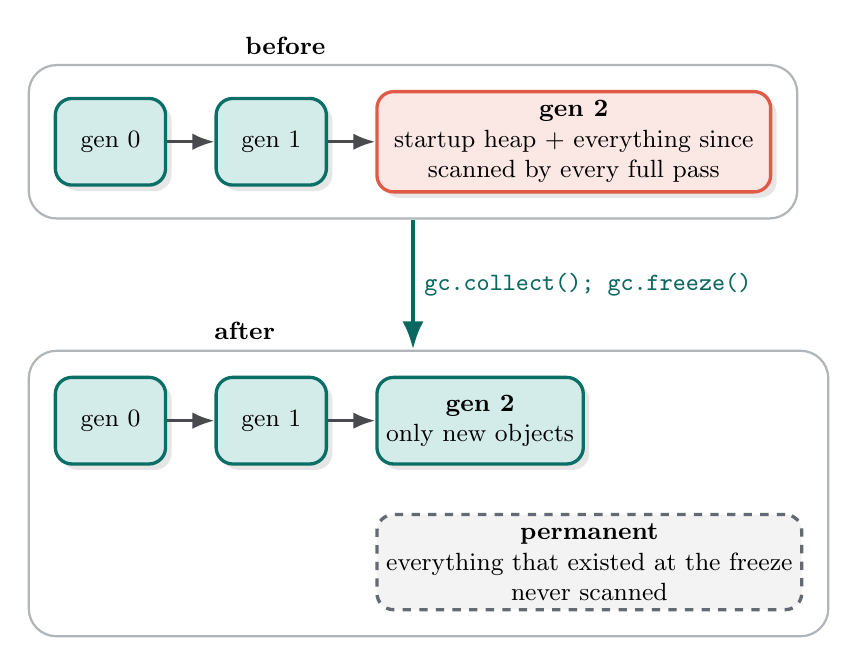
\begin{tikzpicture}[node distance=6mm and 6mm]
  \node[g, minimum width=14mm] (b0) {gen 0};
  \node[g, minimum width=14mm, right=of b0] (b1) {gen 1};
  \node[big, minimum width=50mm, right=of b1] (b2) {\textbf{gen 2}\\startup heap + everything since\\scanned by every full pass};
  \draw[a] (b0) -- (b1);
  \draw[a] (b1) -- (b2);
  \node[frame, fit=(b0)(b2), label={[font=\bfseries\small]above left:before}] (fb) {};

  \node[g, minimum width=14mm, below=24mm of b0] (a0) {gen 0};
  \node[g, minimum width=14mm, right=of a0] (a1) {gen 1};
  \node[g, minimum width=26mm, right=of a1] (a2) {\textbf{gen 2}\\only new objects};
  \node[perm, minimum width=46mm, below=6mm of a2.south west, anchor=north west] (p) {\textbf{permanent}\\everything that existed at the freeze\\never scanned};
  \draw[a] (a0) -- (a1);
  \draw[a] (a1) -- (a2);
  \node[frame, fit=(a0)(a2)(p), label={[font=\bfseries\small]above left:after}] (fa) {};

  \draw[a, draw=acc!70!black, line width=1.6pt] (fb.south) -- node[right, font=\ttfamily\small, text=acc!70!black] {gc.collect(); gc.freeze()} (fa.north -| fb.south);
\end{tikzpicture}
\end{document}
